% Om Project Voldemort
\section{Project Voldemort}

Project Voldemort er et distribuert nøkkelverdilager inspirert av Amazons nøkkelverdilager Dynamo, hvis arkitektur presenteres av \cite{decandia2007}. Dette systemet replikerer og partisjonerer sine data automatisk. Forfatterne og vedlikeholderne \footnote{Kildekoden til Project Voldemort er lisensiert under Apache 2.0 - lisensen, og er tilgjengelig på følgende GitHub-repositorium: \url{http://github.com/voldemort/voldemort/tree/master}} av kildekoden refererer til Voldemort som en stor distribuert, persistent, feiltolerant hash-tabell \citep{kreps2009}. Hver enkelt node i det kjørende databasesystemet holder en delmengde av den totale datamengden som handteres. Flere komponenter i dette systemet, deriblant databasemotoren, plasseringsstrategien for data-tupler, og serialiseringsmetoden, er valgfrie for den enkelte programmerer. Blant annet kan man bruke lagringskomponenter som InnoDB, RocksDB (som benytter LSM-trær), Berkeley DB, eventuelt kan man lagre tupler i primærminnet. I tillegg er også nivået på konsistens av skriveoperasjoner justerbart. Prosessperspektivet til arkitekturen er master-fri, det vil si at i det distribuerte datalageret holdes det ikke valg av spørringskoordinator blant nodene. Derfor opererer de som et likemannsnettverk. Feil som oppstår ved spørringseksekvering behandles transparent.

\subsection{Støttede operasjoner}
Nøkkelverdilagre tilbyr tradisjonelt sett et svært enkelt spørregrensesnitt til applikasjoner som bygger sine datamodeller med dem. Og Voldemort er overhodet ikke annerledes i den forstand. Applikasjonprogrammerings-grensesnittet til Voldemort definerer hovedsakelig tre funksjonelle endepunkter: \texttt{get} (leseoperasjoner), \texttt{put} (skriveoperasjoner, både til opprettelse og oppdatering av tupler), og \texttt{delete} (sletteoperasjoner). I tillegg til disse tre operasjonene som er karakteriske for de fleste nøkkelverdilagre definerer Voldemorts klient – API endepunktene \texttt{getAll}, som er en leseoperasjon på multiple nøkler, og versjonerte utgaver av \texttt{get} og \texttt{put} som til forskjell fra de ordinære funksjonene med samme navn tar inn et versjonsobjekt som input til funksjonen i tillegg til en nøkkel og en verdi, slik at tjeneren slipper å gjøre et oppslag for å finne den nyeste versjonen til det angitte objektet først. Hvis versjonen av objektet hvis nøkkel er spesifisert i funksjonskallet ikke er den nyeste vil klientprogrammet kaste et unntak, kalt \texttt{ObsoleteVersionException}, og brukeren får ingenting returnert. Som tidligere nevnt i den generelle diskusjonen om nøkkelverdilagre anser en databasenode hos Voldemort både nøkkel og det assosierte dataobjekt som en tilfeldig sekvens of bytes. % bryt-opp

% Som et interressant apropos eksponerer \emph{StoreClient} - grensesnittet til Voldemorts kildekode en tredje variant av de to spørringene.  \texttt{get} og \texttt{put}: En variasjon som tar inn en transformsfunksjon som kjøres av databasenodene som mottar disse spørringene før (put) eller etter (get) de oppdater eller henter sitt eget datareplika. Disse funksjonene er nyttige for den som vil implementer en Voldemort-databaseklient i Java som kan migrere data levende hvis det implisitte skjemaet til den ovenstående webapplikasjonen blir endret. % ??

\subsection{Voldemorts egenskaper sammenliknet med RDBMS}
I forhold til relasjonelle databasehåndteringssystemer er Voldemort vesentlig bedre egnet til å innføre replikering av data, da ytelsen til både leseoperasjoner og skriveoperasjoner lar seg skalere horisontalt. Det vil si at hvis en ny node legges til det distribuerte miljøet, også benevnt i litteraturen som ''databaseinstansen'' \citep{sadalage2013}, så vil det ha ingen eller neglisjerbar påvirkning på ytelsen. 

Et relasjonelt DBMS har den fordel over Voldemort at dets innebygde samtidighetshånd\-tering, som utføres ved hjelp av transaksjonsmønsteret, er strengere og derfor mer pålitelig enn Voldemort. Voldemort fokuserer heller på å holde orden på endringshistorikken til hver enkelt tuppel som lagres på den enkelte node i det distribuerte lageret. Ved hjelp av versjonering kan kopier, eller replikaer, av tupler hvis dataverdier er divergerende, rettes opp gjennom en flettingsprosess.

Moderne webapplikasjonssystemer består gjerne av forskjellige, adskilte tjenester eller applikasjonsgrensesnitt, hver av disse kan i sin tur distribuere egne data over opptil flere datasentre rundt om i verden. Slike webapplikasjoner kan ikke ta seg tid til å vente på JOIN - operasjoner mellom to entiteter eller tabeller som potensielt ligger på hver sin MySQL - tjener på hver sin datamaskin i hvert sitt datasenter på to vidt forskjellige lokasjoner på kloden. Én framgangsmåte på å skalere en relasjonell datamodell til å møte behovene til flere tusen forespørsler samtidig, er å introdusere et hurtiglager-nivå i systemarkitekturen ved hjelp av et distribuert, minnebasert cachesystem som MemCache eller Redis. Dette hurtiglageret avlaster databasen for leseoperasjoner, som vil utgjøre en flaskehals for den samlede ytelsen til den distribuerte applikasjonen. Dessverre vil ikke denne løsningen skalere for skriveoperasjoner og JOIN - operasjoner så lenge logisk konsistens for skrivinger er et krav. Voldemorts løsning, hvis tekniske detaljer vil bli diskutert i neste delkapittel, er å lempe på disse konsistenskravene.

Relasjonelle databasesystemer realiserer de assosiasjoner som er spesifisert mellom entitetene i datamodellen til applikasjonens arkitektur. Relasjonelle databasesystemer oppfyller samtidig fire egenskaper for skriveoperasjoner som gjøres i systemet gjennom transaksjonsmønsteret. Atomisitet, en garanti på at hver enkelt transaksjon enten utføres fullt og helt eller avbrytes; Konsistens: for hver enkelt utførte transaksjon etterlates databasen i en konsistent tilstand; Isolasjon: Hver enkelt transaksjon kjøres uavhengig av hvilke andre transaksjoner som kjøres samtidig; Holdbarhet: Data som er persistert gjennom transaksjoner i systemet, vil ikke endres eller forsvinne med mindre påfølgende transaksjoner gjør det. Hver enkelt PUT-operasjon i Voldemort er atomisk så lenge den opererer på et og samme aggregat i datamodellen, det vil si den komplekse objektverdien som aksesseres med nøkkelen.

Transaksjoner gjør skriveoperasjoner i relasjonelle databaser lineariserbare, som er det strengeste konsistensnivået skriveoperasjoner kan ligge på i databasesystem, ved å tvinge skriveoperasjonen til å vente hvis den prøver å endre rader eller tabeller som allerede er reservert for en tidligere påbegynt transaksjon. Voldemort, på sin side legger seg på et mildere konsistensnivå, kalt svak konsistens (eng. ''eventual consistency'').

\subsection{Konsistenskontroll og versjonering}
I likhet med Amazon Dynamo er også Voldemort sin replikakonsistenskontroll inspirert av quorumsystemer. Quorumreplikering og Dynamos liknende replikeringsstrategi av det beskrives i \ref{dynark}.

På samme vis som i Dynamo tillater Voldemort samtidige skriveoperasjoner på samme nøkkel på forskjellige noder. Begrunnelsen for dette valget er at Dynamo er alltid mottakelig for skriveoperasjoner \citep{decandia2007}, slik at for eksempel en handlekurv alltid kan oppdateres i sanntid. Følgelig kan to eller flere replikaer for samme nøkkel være lagret på forskjellige noder, uten å være synkroniserte. Det vil si at ingen av de to replikaene har den fulle og hele oppdateringshistorikken til nøkkelen. I stedet for å preservere replikakonsistens i systemet for alle nøkler til enhver tid, går både Dynamo og Voldemort for å forsone divergerende replikaer for en og samme nøkkel når den blir \texttt{get}-et av applikasjonen, en prosess kalt ''read repair'' av \cite{decandia2007}.

Hvert dataobjekt som skrives tillegges en vektorklokkeverdi som del av dets metadata. Ved en leseforespørsel på samme nøkkel kan koordinatoren for denne leseforespørselen motta replikaer med divergerende vektorklokkeverdier, også kalt \emph{versjoner} \citep{kreps2009}. Hvis systemet er i stand til å forsone og flette oppdateringshistorikken til nøkkelen basert på vektorklokkeverdiene til replikaene, så vil spørringskoordinatoren returnere én gjeldende dataverdi tilbake til klienten som sendte leseforespørselen. Samtidig vil koordinatoren sende skrivespørringer til hver av replikanodene til nøkkelen slik at de kan oppdatere sitt replikaobjekt med den flettede verdien.

Hvis en fletteoperasjon ikke er mulig å utføre med bare vektorklokker, vil spørrings\-koordinatoren returnere alle de konflikterende versjonene av aggregatet til applikasjonsklienten, slik at den selv kan flette den sammen. Applikasjonen vil deretter persistere den definitive, sammenflettede versjonen av aggregatet tilbake til datalageret.

\subsection{Serialisering av dataobjekter}
Innen datateknologi er serialisering prosessen der objekter eller datastrukturer i datamaskinminne som holder på applikasjonsdata, konverteres til et format som lar seg lagres på disk, eventuelt forsendes over et nettverk. I en datamaskins interne minne kan dataobjekter som aksesseres av en og samme programvareprosess, ligge på vidt forskjellige minneadresser. Hvis disse dataobjektene skal forsendes over et I/O - grensesnitt, er det viktig å samle dem sammen og ordne dem på et vis som kan leses av en datamaskin, derav begrepet serialisering. Serialisering går som regel ut på å flatpakke en nøstet datastruktur, for eksempel et tre, et objekt, eller en matrise, til en enkelt-dimensjonal sekvens av binære sifre. Den konverterte strengen av bits blir da enten persistert til disk eller sendt til en helt annen datamaskin over et IP - nettverk. Ved mottak eller lesing fra disk, blir bit-strengen konvertert tilbake til den opprinnelige datastrukturen. Serialisering kan også brukes i eksterne prosedyrekall (RPC).

Serialisering av minnebaserte datastrukturer er en ganske vanlig oppgave i distribuerte systemer og applikasjonsprotokoller, og derfor kan dette gjøres i mange programmeringsspråk. I Java blir klasser som implementerer grensesnittet java.io.Serializable automatisk serialisert. I Python brukes modulen pickle fra standardbiblioteket til samme formål. I PHP nyttes funksjonen \texttt{serialize()} til serialisering og \texttt{unserialize()} til parsing. I JavaScript er JSON - objektet, med dets to metoder \texttt{parse()} og \texttt{stringify()} innebygd i språket. JSON - protokollen er nemlig basert på et subsett av JavaScript. Følgelig kan en hvilken som helst datastruktur formet i JSON - syntaksen oversettes til JavaScript - syntaks.

Hos Voldemort serialiseres dataobjekter før de lagres. Ved å serialisere data kan man garantere at datalageret er helt og holdent uvitende om hva det er sekvensene av 1-ere og 0-ere som blir lagret står for. Applikasjonsutviklere som benytter Voldemort som sin database, kan bruke en av mange forskjellige teknikker, eventuelt implementere sin egen. Serialisering sies å være -pluggbart- i Voldemort, slik at man står fritt til å bruke serialiseringsrammeverk som Apache Avro, Googles ProtoBuf, Apache Thrift og Javas serialiseringsgrensesnitt som tidligere nevnt \citep{kreps2009}. Ved hjelp av serialisering kan komplekse datastrukturer, som lister og navngitte tupler, benyttes både som nøkler og verdi for de enkelte rader. Et siste konfigurasjonsalternativ som kan nevnes er ''string''-serialisering. Dette alternativet benyttes hvis databaseklienten mottar preformatert data på strengform, og er dermed fullstendig skjemaignorant.

\subsection{Lastbalansering av dataobjekter}

I et klynget databasesystem er det viktig å fordele datareplikaer, slik at hver node i klyngen holder på omtrent like stort datavolum til enhver tid. For skalerbarheens skyld kan ikke én eneste node holde på samtlige dataobjekter som lages i databasen, ellers vil datautilgjengeligheten være inversproporsjonal med antallet tjenere i klyngen.

% Konsistent hashing i implementasjon av Voldemort
Konsistent hashing - teknikken brukes også i Voldemorts lastbalanseringsalgoritme. I likhet med Amazon Dynamo er konsistent hashing en viktig algoritme som brukes for å oppnå jevn fordeling av nøkler. I tillegg er konsistent hashing involvert i både replikering og rebalansering av datalasten, noe en enkel hashfunksjon ikke kan gjøre. En vanlig hashalgoritme hasher data eller nøkler inn i binært rom bestående av et fast, forhåndsinnstilt antall \emph{partisjoner}, eller bøtter. Hver av disse partisjonene handterer et forhåndsinnstilt del av det binære verdiområdet (et tall fra 0 til en stor toerpotens minus 1) til hashfunksjonen. % +++

% Ved svikt i node
Når en node svikter permanent, vil datalasten bli omdistribuert til de gjenværende nodene i ringen, hvis partisjoner grenser mot de partisjonene av ringen den feilede noden hadde ansvar for, altså omadresseres aggregater tidligere lagret av en nå feilet og permanent utilgjengelig node. Noder med høyere lagringskapasitet lagrer flere datatupler fordi de har ansvar for en større brøkdel av ringen av diskrete hashverdier. % bryt-opp

% Figur 4
\begin{figure}[!ht]
    \centering
    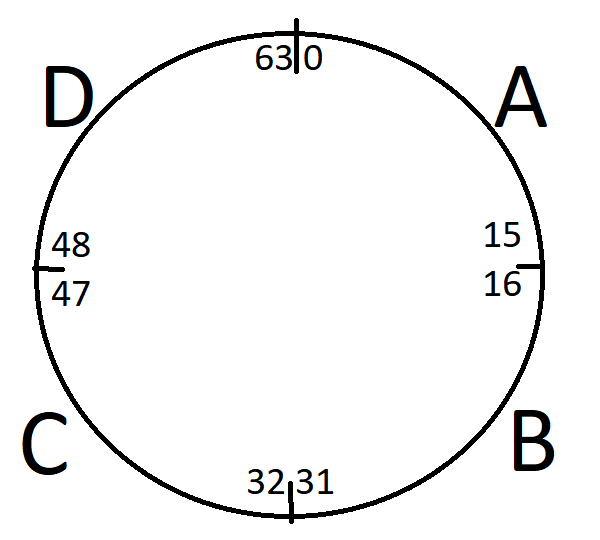
\includegraphics{fig/hashring.png}
    \caption{Eksempel på konsistent hashring i Project Voldemort.}
    \label{fig4}
\end{figure}

Den logiske strukturen til likemannsnettverket av databasenoder i Voldemort har formen til en ring. Denne ringen består av en stor mengde diskrete posisjoner, verdiområdet til en hashfunksjon \emph{h}. Hver node som deltar i databaseklyngen, tildeles en gruppe av disse punktene i ringen. \emph{h} brukes til å finne ringposisjonen til en nøkkel \emph{k}. Den noden, hvis tilordnede mengde av hashverdier inneholder \emph{h(k)}, blir den som lagrer det assosierte dataobjektet til \emph{k}.

Den konsistente hashalgoritmen og ringstrukturen til likemannsnettverket realiserer datareplikering ved å legge antallet påkrevde replikaer, per quorumkonfigurasjonen, på etter-følgende noder i ringen, med sola \citep{elmasri2014}. Per figur \ref{fig4} og replikakonfigurasjonen \(N=3\) vil eksempelvis alle dataobjekter som hashes til node A, også kopieres til node B og C. Av denne figuren kan man lese at node A lagrer nøkler med hashverdi 0-15, B lagrer nøkler hvis hashverdi er mellom 16 og 31, C lagrer nøkler hvis hashverdi er mellom 32 og 47, og D lagrer nøkler hvis hashverdi er mellom 48 og 63.

